Note: there are more plots inside the folders that were used to tune the parameters. Due to the space limit, I did not show them in the report.

\section{Problem 1}

\subsection{Data statistics and plot}

\begin{figure}[H]
\centering
  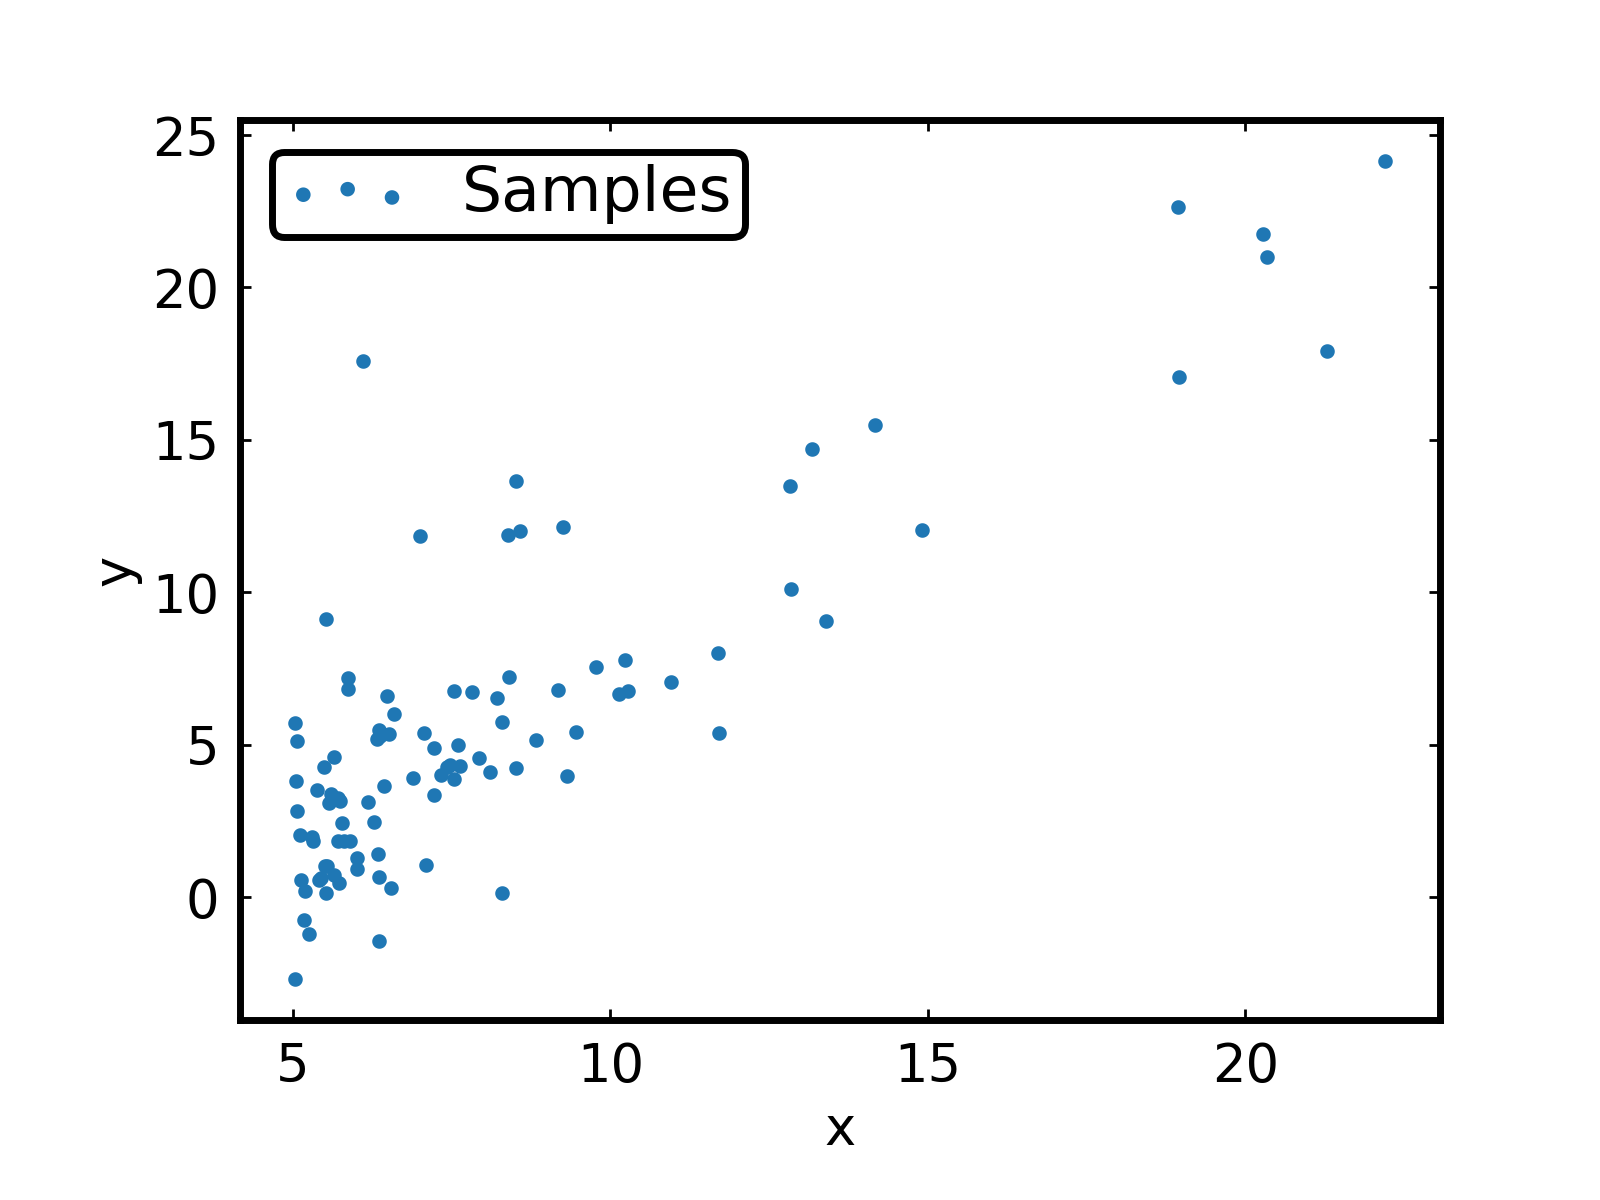
\includegraphics[width=0.85\textwidth]{fig/prob1/data.png}
\centering 
\caption{Data}
\label{fig:data}
\end{figure}

\subsection{Result}

With the parameter as $alpha = 0.001$, $eps = 10^{-8}$, 
$n_{epoch} = 10000$, we can get the regression with final loss as 4.516. The learned parameters are 

\begin{equation}
w = 1.127, b = -3.240
\end{equation}

\begin{figure}[H]
\centering
  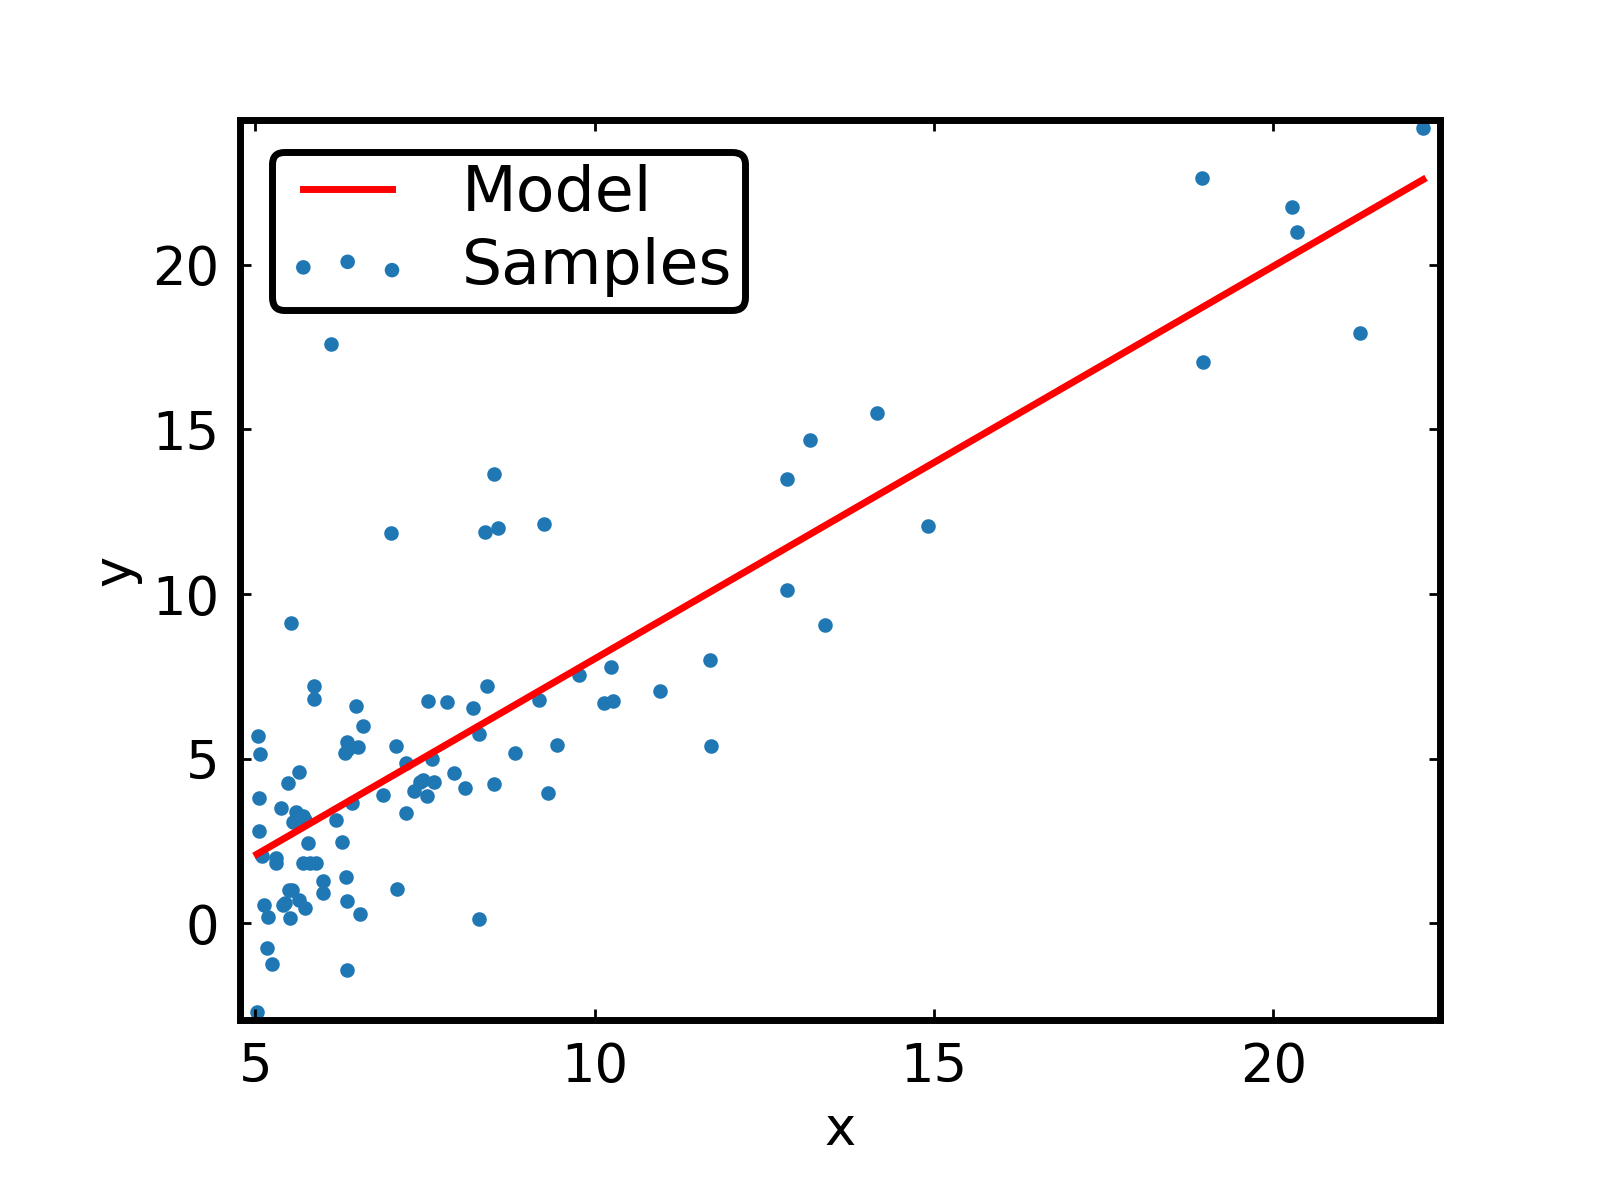
\includegraphics[width=0.85\textwidth]{fig/prob1/fit.png}
\centering 
\caption{Fitting result v.s. data}
\label{fig:fit}
\end{figure}

\begin{figure}[H]
\centering
  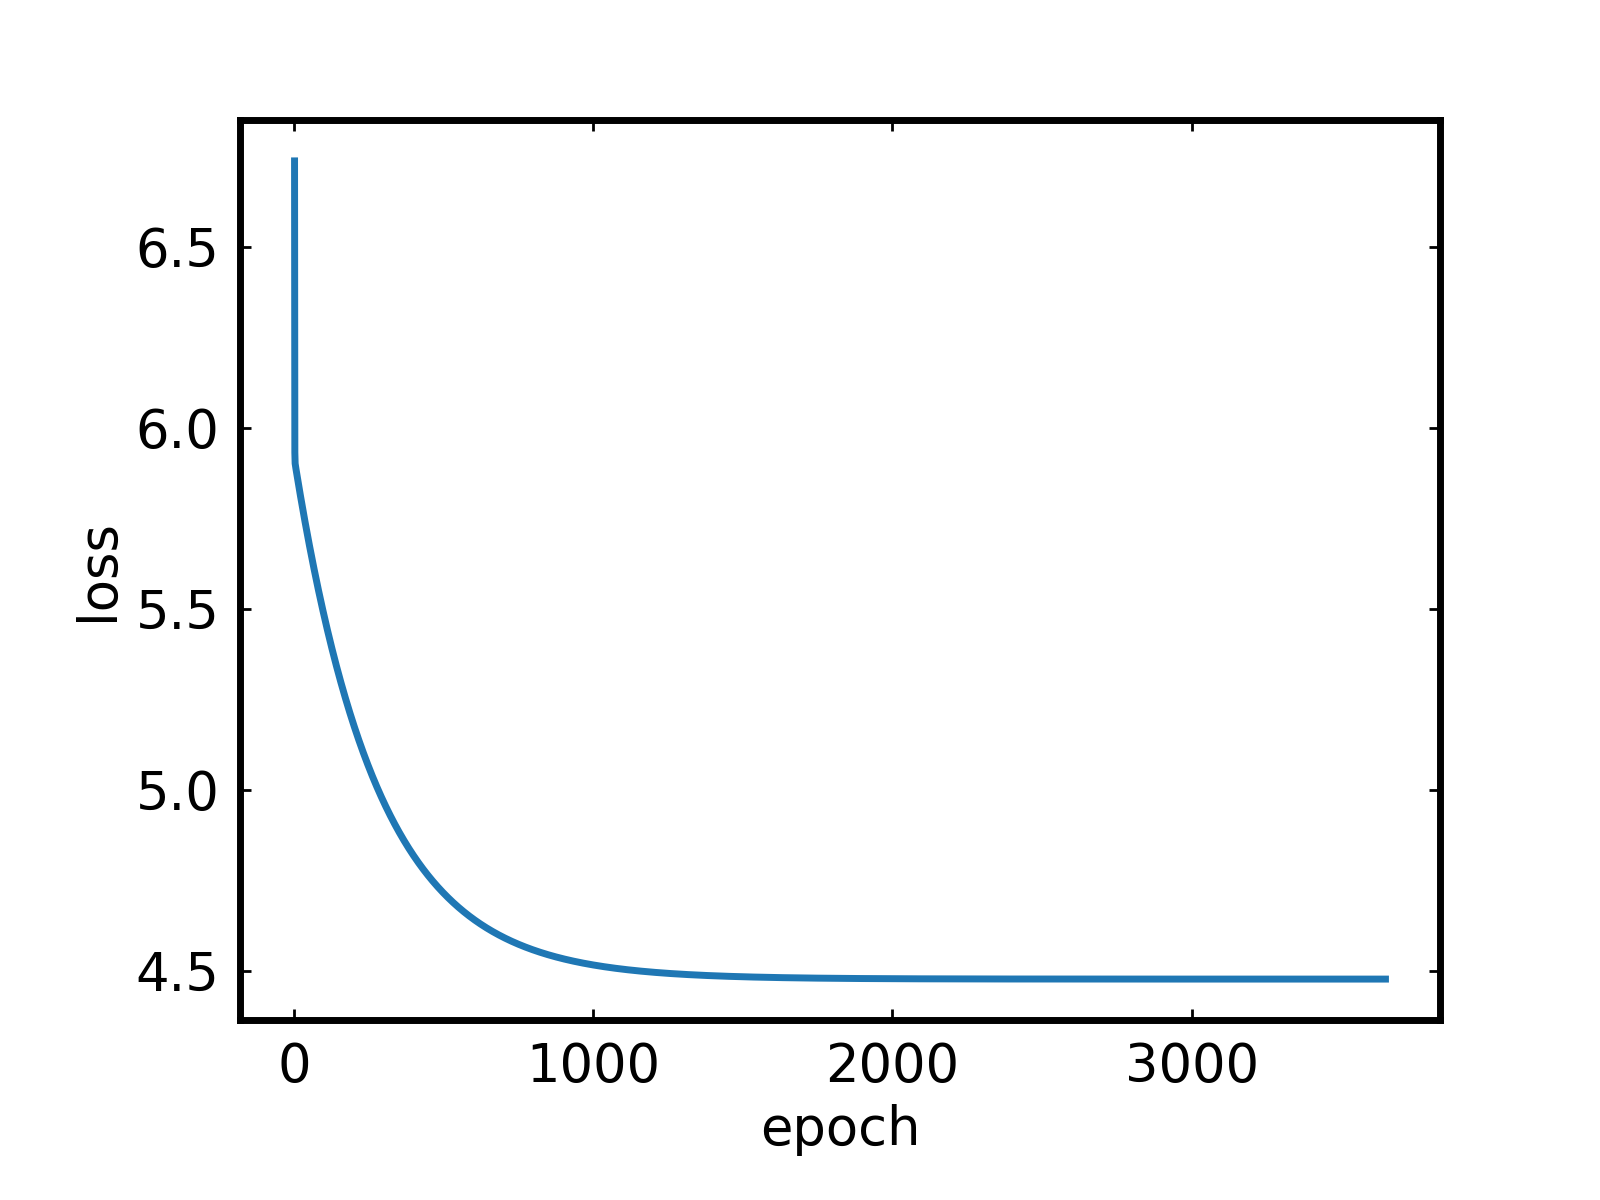
\includegraphics[width=0.85\textwidth]{fig/prob1/loss.png}
\centering 
\caption{Loss v.s. epochs}
\label{fig:loss}
\end{figure}

Here is the process of tuning the parameter alpha. 

\begin{table}[htb]
\centering
\caption{Loss for different learning rate alpha}
\begin{tabular}{|l|l|}
\hline
$\alpha$ & loss \\ \hline
0.0001 & 5.48 \\ \hline
0.001 & 4.51 \\ \hline
0.01 & 4.47 \\ \hline
0.02 & 4.47 \\ \hline
0.05 & nan \\ \hline
0.1 & nan \\ \hline
\hline
\end{tabular}
\label{tab:alpha}
\end{table}

Small learning rate will make the learning process very slow. For example, when $\alpha$ is set to 0.0001, after 10,000 epochs, the loss is still decreasing. Larger learning rate will speed up the learning process, but may lead to unstable results. Usually, it takes several hundreds (\~500) epochs to converge to a reasonable solution.

